\documentclass[tikz,border=5pt]{standalone}
\usepackage{amsmath,amssymb}
\usetikzlibrary{arrows.meta,positioning,calc,fit,backgrounds}

\newcommand{\pseudo}[1]{%
  \begin{scope}[on background layer]
    \fill[black!20] ($(#1.south east)+(0.18,0.12)$) -- ($(#1.north east)+(0.18,0.12)$)
      -- (#1.north east) -- (#1.south east) -- cycle;
    \fill[black!10] ($(#1.north west)+(0.18,0.12)$) -- ($(#1.north east)+(0.18,0.12)$)
      -- (#1.north east) -- (#1.north west) -- cycle;
    \draw[line width=0.35pt, black!55] ($(#1.north west)+(0.18,0.12)$)
      -- ($(#1.north east)+(0.18,0.12)$) -- ($(#1.south east)+(0.18,0.12)$);
    \draw[line width=0.35pt, black!55] (#1.north east) -- ($(#1.north east)+(0.18,0.12)$);
    \draw[line width=0.35pt, black!55] (#1.south east) -- ($(#1.south east)+(0.18,0.12)$);
  \end{scope}%
}

\begin{document}
\begin{tikzpicture}[
  >={Stealth[length=2mm]},
  box/.style={draw, rounded corners=2pt, align=center, font=\footnotesize,
              inner sep=3pt, minimum height=8mm, line width=0.5pt},
  input/.style={box, fill=blue!6},
  enc/.style={box, fill=blue!14},
  scal/.style={box, fill=orange!12},
  spec/.style={box, fill=green!10},
  fus/.style={box, fill=black!7},
  pred/.style={box, fill=violet!12},
  dec/.style={box, fill=orange!8},
  outbox/.style={box, fill=white, line width=0.9pt},
  teach/.style={box, fill=white, dashed, draw=black!60},
  lossbox/.style={box, fill=yellow!10},
  ar/.style={->, line width=0.55pt, black!85},
  tarr/.style={->, dashed, line width=0.55pt, black!60},
  band/.style={draw=black!25, dashed, rounded corners=6pt, inner sep=10pt},
  lab/.style={font=\scriptsize, inner sep=1pt, black!70},
]

% ---------------- inputs ----------------
\node[input, inner sep=1pt] (occ) at (0, 1.9) {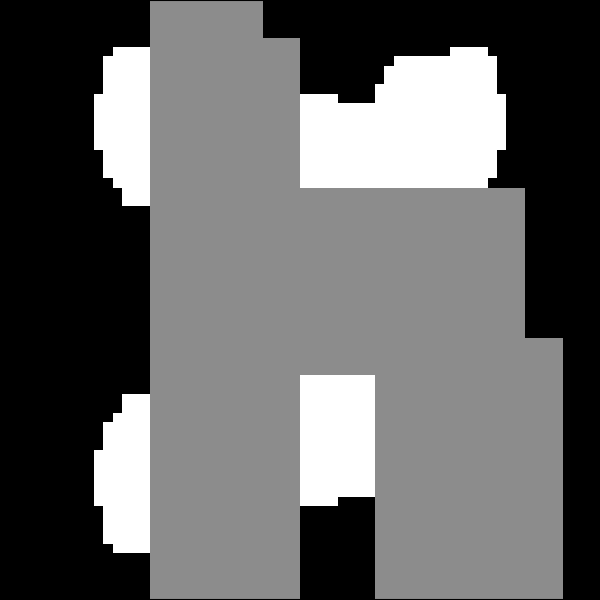
\includegraphics[width=11mm]{occ_masked.png}};
\node[lab, below=0pt of occ] {masked $G$};
\node[input] (spe) at (0, 0) {spectrum\\$[B,2,301]$};
\node[input] (par) at (0,-1.9) {parameters\\$[B,6]$};

% ---------------- encoders ----------------
\node[enc]  (oe) at (3.5, 1.9) {occupancy encoder\\patch $4\!\times\!4$, 6 blocks + FiLM};
\node[spec] (pe) at (3.5, 0)   {frozen spectrum\\encoder};
\node[scal] (se) at (3.5,-1.9) {scalar MLP\\$6\!\to\!128\!\to\!128$};

% ---------------- read-out: goal tokens only ----------------
\node[spec, minimum height=5.5mm] (ag) at (6.0, 0) {$\mathbf{a}$};
\node[lab, above=1pt of ag] {16 goal tokens};

% ---------------- fusion, predictor ----------------
\node[fus, minimum height=50mm] (fu) at (8.1,-0.15) {fusion\\2 layers\\$273\times192$};
\node[pred, minimum height=14mm] (gc) at (11.2,-0.15) {GCLCT\\8 blocks};

% ---------------- global condition, drawn after fusion ----------------
\node[spec, minimum height=5.5mm] (cf) at (11.2,-3.4) {$\mathbf{c}$};
\node[lab, above=1pt of cf] {global physics};

% ---------------- decoders and outputs ----------------
\node[dec, align=center] (od) at (14.4, 1.15) {occupancy decoder\\$192\!\to\!96$ FiLM: $16^2\!\to\!32^2$\\$2\times$ FiLM blocks at $32^2$\\$3\times3$ head $\Rightarrow 64^2$};
\node[dec] (sd) at (14.4,-1.7) {scalar decoder\\$192\!\to\!64\!\to\!3$};
\node[outbox] (des) at (17.7, 1.15) {design $\hat G$\\$64\times64$};
\node[lab, below=2pt of od, align=center] {variant: $32^2$ quadrant $\Rightarrow$ mirror};
\node[outbox] (prm) at (17.4,-1.6) {$\hat l,\hat h,\hat r$};

% ---------------- teacher ----------------
\node[input, inner sep=1pt] (occf) at (0,-5.8) {
\includegraphics[width=11mm]{occ_sample.png}};
\node[lab, below=0pt of occf] {full $G$};
\node[input] (parf) at (0,-7.5) {all parameters\\known};
\node[teach] (toe) at (3.5,-5.8) {EMA occupancy\\encoder $+$ frozen\\spectral FiLM};
\node[teach] (tse) at (3.5,-7.5) {EMA scalar MLP\\$\to$ FiLM};
\node[outbox] (tgt) at (8.1,-5.8) {$\mathbf{z}_y^{\mathrm{spec}}$\ \ $\mathbf{z}_y$\\$\mathbf{z}_y^{\mathrm{sc}}$};
\node[lossbox] (lss) at (11.2,-5.8) {$\mathcal{L}_{\mathrm{inv}},\mathcal{L}_{\mathrm{var}},\mathcal{L}_{\mathrm{cov}}$\\$\mathcal{L}_{\mathrm{cond}},\mathcal{L}_{\mathrm{scal\text{-}t}}$};

% ---------------- student edges ----------------
\draw[ar] (occ) -- (oe);
\draw[ar] (spe) -- (pe);
\draw[ar] (par) -- (se);

\draw[ar] (pe.east) -- (ag.west);
\draw[ar] (ag.east) -- (fu.west |- ag.east);
\draw[ar] (oe.east) -- (fu.west |- oe.east);
\draw[ar] (se.east) -- (fu.west |- se.east);

\draw[ar] (fu.east) -- (gc.west);
\draw[ar] (gc.east) -- ++(0.40,0) |- (od.west);
\draw[ar] (gc.east) -- ++(0.40,0) |- (sd.west);
\draw[ar] (od) -- (des);
\draw[ar] (sd) -- (prm);

% c: same read-out, routed under the fusion block, then into GCLCT as FiLM
\draw[ar] (pe.east) -- ++(0.55,0) -- ++(0,-3.4) -- (cf.west);
\draw[ar] (cf.north) -- (gc.south);

% ---------------- teacher edges ----------------
\draw[tarr] (occf) -- (toe);
\draw[tarr] (parf) -- (tse);
\draw[tarr] (toe) -- (tgt);
\draw[tarr] (tse.east) -- ++(0.6,0) |- (tgt.west);
\draw[tarr] (tgt) -- (lss);
\draw[tarr] (gc.east) -- ++(0.40,0) -- ++(0,-4.9) -| (lss.north);
\draw[tarr] (cf.south) -- ++(0,-0.9) -| ([xshift=-9mm]toe.north);
\coordinate (filmTop) at ({1.30},2.70);
\draw[tarr] (se.west) -- ({1.30},-1.9) -- (filmTop) -- ({3.5},2.70) -- (oe.north);

% ---------------- bands ----------------
\coordinate (sNE) at ($(des.north east)+(0.36,0.28)$);
\coordinate (sSW) at ($(par.south west)+(-0.22,-0.26)$);
\coordinate (tNE) at ($(lss.north east)+(0.36,0.28)$);
\coordinate (tSW) at ($(parf.south west)+(-0.22,-0.26)$);
\begin{scope}[on background layer]
\node[band, fit=(occ)(par)(spe)(oe)(se)(pe)(ag)(fu)(gc)(cf)(od)(sd)(des)(prm)(sNE)(sSW)] (sband) {};
\node[band, fit=(occf)(parf)(toe)(tse)(tgt)(lss)(tNE)(tSW)] (tband) {};
\end{scope}
\node[lab, anchor=south west] at ([yshift=1pt]sband.north west) {student, inference path};
\node[lab, anchor=south west] at ([yshift=1pt]tband.north west) {teacher, training only, no gradient};

% ---------------- pseudo-3D ----------------
\foreach \n in {occ,spe,par,oe,pe,se,ag,fu,gc,cf,od,sd,des,prm,occf,parf,toe,tse,tgt,lss} {
  \pseudo{\n}
}

\end{tikzpicture}
\end{document}
